% !TEX program = xelatex

\section{Data preparation}
% TODO: What was the correct term for this?

\iffalse{}
\subsection{Normalization}
\fi

\subsection{3D and 2D Annotations}

% TODO: "mention first how were 2D annotations created. Why only 2D? -> trade-off time consumption vs. value"
% TODO: Why this approach for 3D-reconstruction?
% Inital thoughts: 
%  - Most current algorithms are ML-based.
%  - Some require medical knowledge
%  - Too few 3D annotations to check/train ML model
%  - Is it a good idea to base ML model on another ML model?
% Read "auto_vs_semiauto_vs_manual_anno.pdf" when not half asleep. Even "automatic" seems
% to require human intervention(?).
% ~prostate_automatic_annotation.pdf seems to suggest ellipsoid a-priori shape for tumors.~
% Misunderstanding: shape of prostate (not tumor!) was described

While all \ac{mri} scans in the dataset consist of 3-dimensional data, 
most are segmented along only 2 axes, forming a flat slice in the scan.
An example would be an annotation that cover only the sagittal plane. 
Note, that the annotation file for 
a 2-dimensional annotations is still a 3-dimensional image, but the 
\ac{roi} is marked only in one slice, as can be seen in Figure~\ref{fig:2dvs3d}.

\begin{figure}[H]
    \centering
    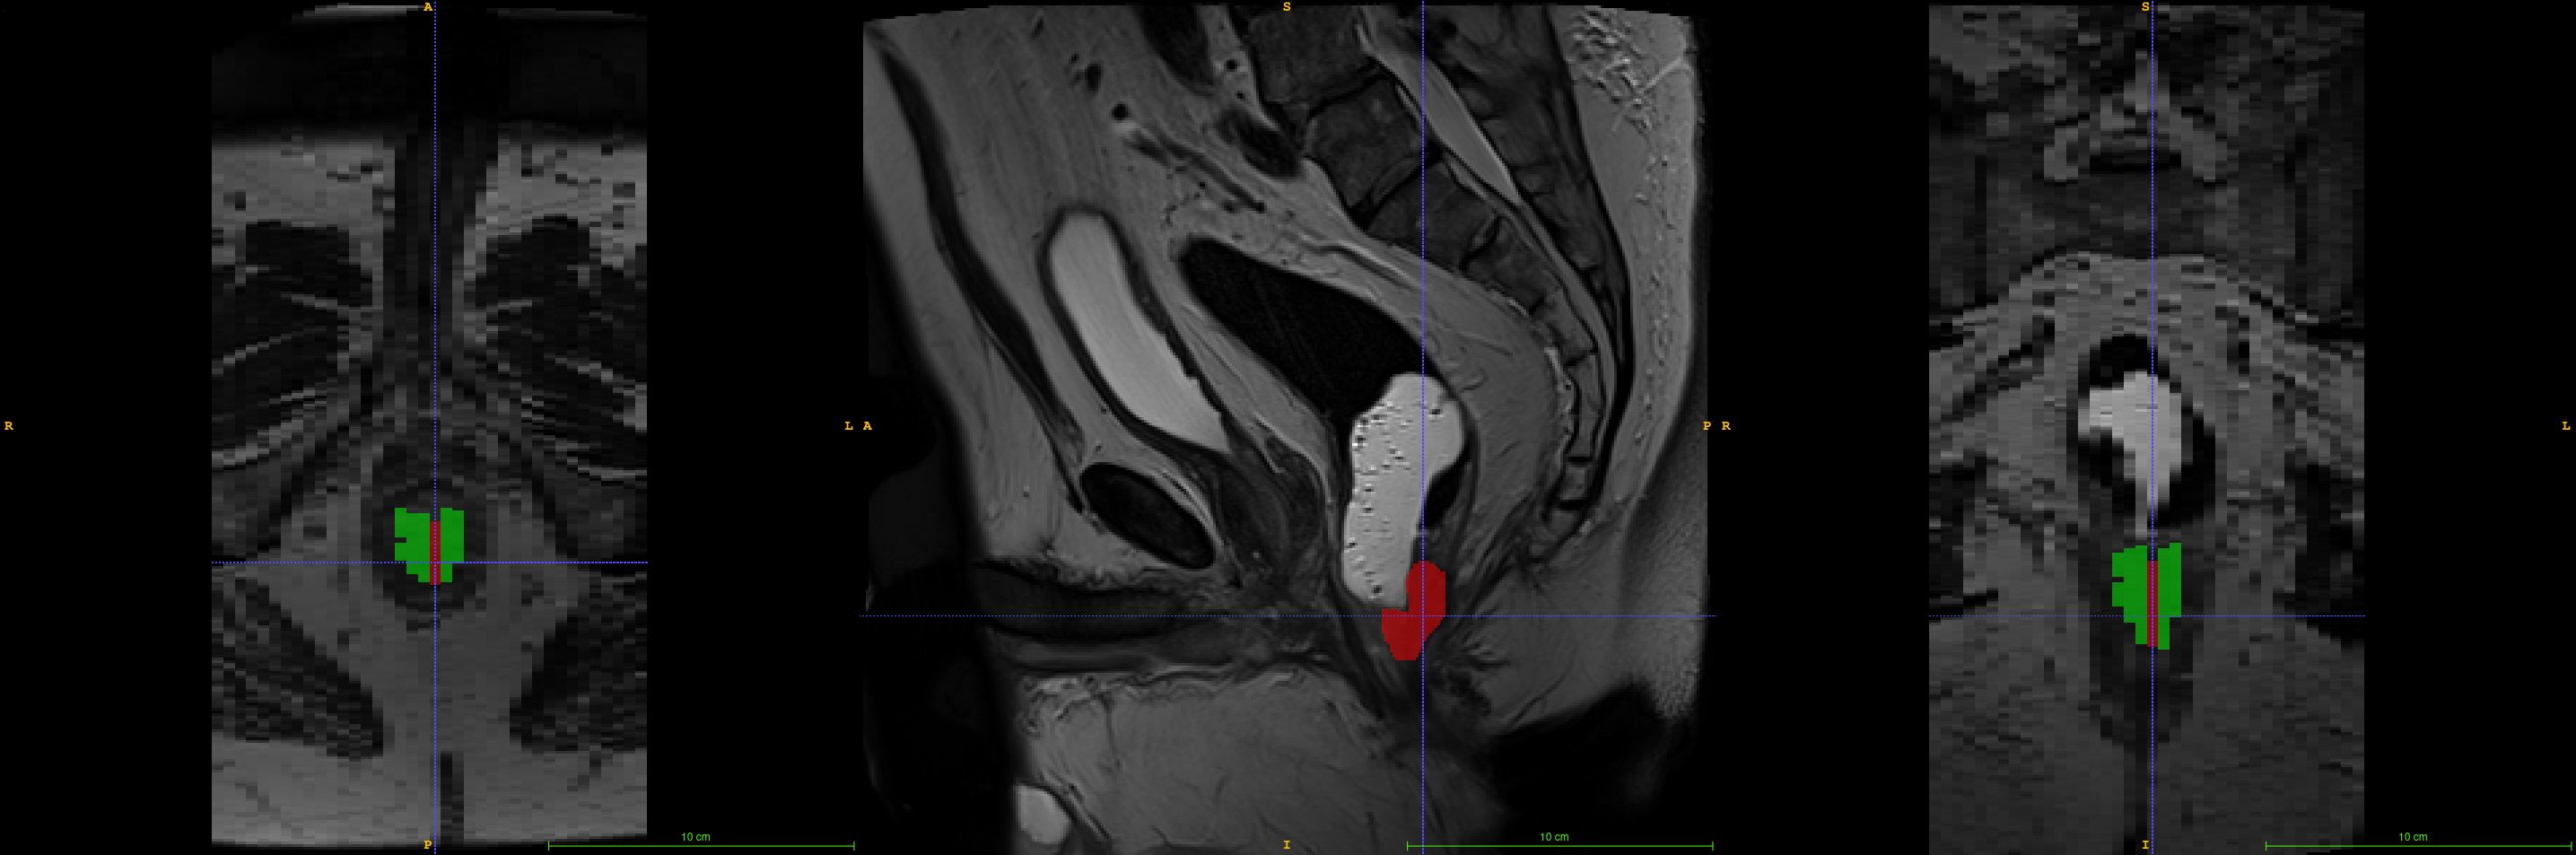
\includegraphics[width=1.0\textwidth]{img/mo0501229884a_marked.png}
    \caption{A manual tumor annotation. A 2-dimensional annotation is marked in red. As it is formed by voxels, it still possesses a non-zero width. If combined with the annotation marked in green, it forms a 3-dimensional annotation. From right to left: axial plane, sagittal plane and coronal plane.}\label{fig:2dvs3d}
\end{figure}

For ease of understanding, 
2-dimensional annotations will be treated as 2-dimensional images, if not
noted otherwise.
This mixture of annotation types poses a set of problems; requirements of radiomics
features and consistency. A group of PyRadiomics' features, namely 
\enquote{Shape Features (3D)} rely on a 3-dimensional \ac{roi}. With a largely 2-dimensional
dataset, these features would need to be excluded. Furthermore, it has been suggested, 
that analysis of complete tumors may be more representative
of a tumor's features than analysis of its biggest slice, especially in colorectal 
tumors~\cite{whole_tumor_vs_cross_section}\cite{rad_in_prec_med}.
In contrast, some scans in the dataset are annotated along 3 dimensions. 
This inconsistency in input data may lead to varying ratios of 2D and 3D 
annotated data in subsamples, strongly impacting reproducibility.

\subsubsection{Creation of 2D annotations.}
% Describe 2D-ification
As all 3D annotations in the dataset were created manually, they can neither
be recreated automatically nor reliably, without involving the original annotators.
To avoid a mix of manual and automated 3D annotations, the same 3D reconstruction 
algorithm will be applied to all annotations.
Manual 3D annotations will therefore treated as 2D annotations 
and must be reduced by one axis.

To lose as little information as possible, while still dropping information along the third
axis, the largest area along two axes in the 3D annotation is used. To determine this slice
of the original annotation, the annotation is split into 2-dimensional slices along each axis.
For each slice, all marked voxels marked as part of the \ac{roi} can be counted. As the axes of 
these voxels may be unevenly scaled, the voxel count must be multiplied with a correction factor to account for
the different axis scales. The largest area after application of the correction factor is the 
largest 2D-slice by area, and therefore the new 2D annotation.

\subsubsection{Creation of 3D annotations.}
% Describe inverse distance transform + optimization steps
% Now, the fully 2D-annotated dataset can be converted to 3D annotations.
Now, 3D annotations can be reconstructed from the fully 2D annotated dataset.
The algorithm used here was chosen to be simple to implement and reproduce.
It is based on \enquote{inverting} a 2-dimensional euclidean distance 
transformation. % Don't forget to include the figure


The distance transform assigns each pixel in an image a value based on the
pixel's distance to the nearest pixel with a non-zero color 
value~\cite{2020SciPy-NMeth}. Here, the distance is determined by the 
L\textsubscript{2} norm, adjusted for potentially uneven scaled axes. As 
demonstrated in Figure~\ref{fig:2d-annotation} using this transformation on a 
2-dimensional annotation yields the distance of each pixel inside the 
\ac{roi} to the nearest pixel outside the \ac{roi}. This property will 
henceforth simply be referred to as a pixel's \enquote{2D distance}.

\begin{figure}[H]
    \centering
    \begin{subfigure}[t]{0.4\textwidth}
        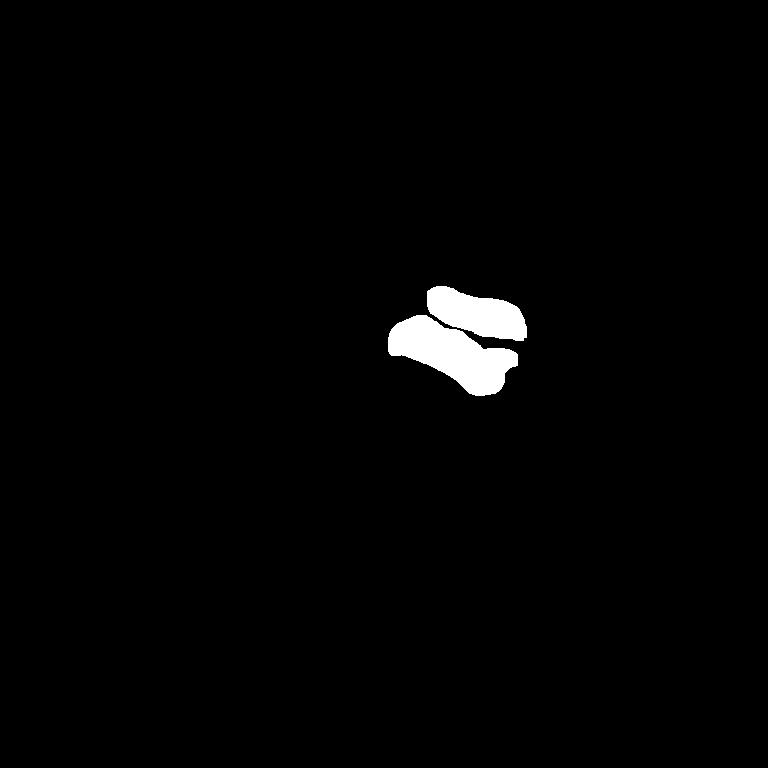
\includegraphics[width=\textwidth]{img/img_base_mr1a.jpg}
        \caption{Base image. White areas mark the \ac{roi}.}\label{fig:2d-base}
    \end{subfigure}
    ~
    \begin{subfigure}[t]{0.4\textwidth}
        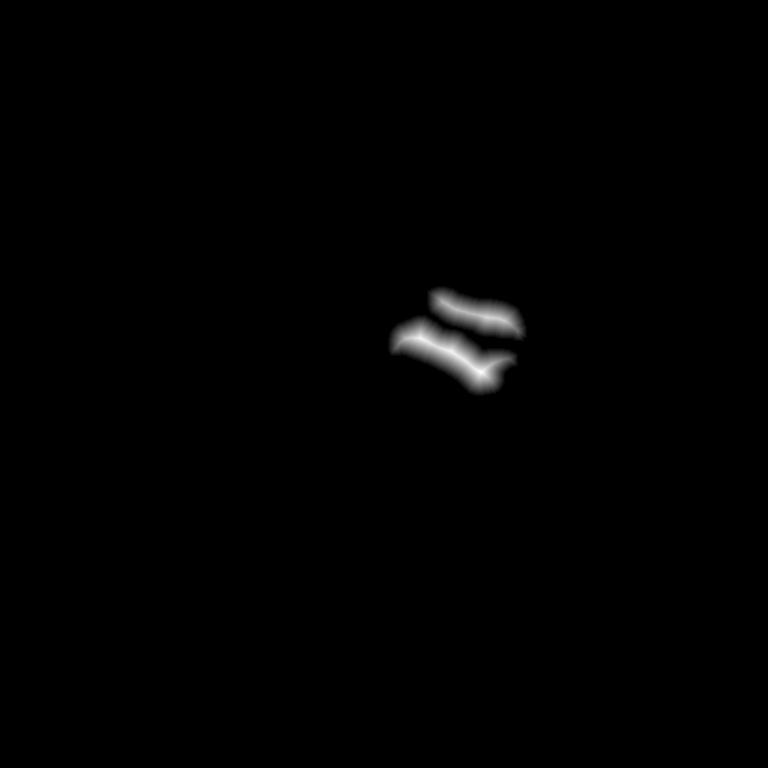
\includegraphics[width=\textwidth]{img/img_dist_mr1a.jpg}
        \caption{Euclidean distance transform implemented by~\cite{2020SciPy-NMeth}. Lighter colors indicate a greater distance.}\label{fig:2d-dist}
    \end{subfigure}
    \caption{A 2-dimensional \ac{roi} annotation. The contrast of both images has been increased to allow for easier viewing.}
    \label{fig:2d-annotation}
\end{figure}

% Draft 1
% To create a 3-dimensional annotation, new layers of pixels along the new
% third axis will be added. If any new pixel is closer to a pixel that is 
% part of the original \ac{roi} than the original pixel's 2D distance (as 
% determined by the distance transformation), the new pixel is also made part
% of the \ac{roi}.

% Draft 2
To create a 3-dimensional annotation, new layers of voxels along the new
third axis will be added. The distance of each new voxel in relation to 
every pixel in the original \ac{roi} is determined. Should the 
\enquote{2D distance} of a pixel in the \ac{roi} be larger than the 
distance between that pixel and the new voxel, the new voxel is added to 
the new \ac{roi}. A pseudo-code implementation of this algorithm is shown
in Listing~\ref{code:3dpseudo}.

\begin{lstlisting}[caption=3D reconstruction., label={code:3dpseudo}]
    annotation_2d = get_largest_slice(annotation_original)
    annotation_2d_distances = euclidean_distance(annotation_2d)

    for voxel_new in annotation_new:
        for pixel_old in annotation_2d:
            if euclidean_distance(voxel_new, pixel_old) <= annotation_2d_distances[pixel_old]:
                annotation_new[voxel_new] = 1
                break

\end{lstlisting}

This leads to a new 3-dimensional annotation, symmetrical along the initial
2-dimensional annotation slice. As can be seen in Figure~\ref{fig:3d-annotation},
the thickness of the annotation increases with the \enquote{2D distance} of 
the underlying pixels. Should the 2-dimensional annotation along the base 
layer be circular, the 3-dimensional annotation will approach a sphere.



% Describe check for new pixels (is this pixel along the 3rd axis closer
% than roi pixel's distance? -> Include in roi.)


\begin{figure}[H]
    \centering
    \begin{subfigure}[t]{0.4\textwidth}
        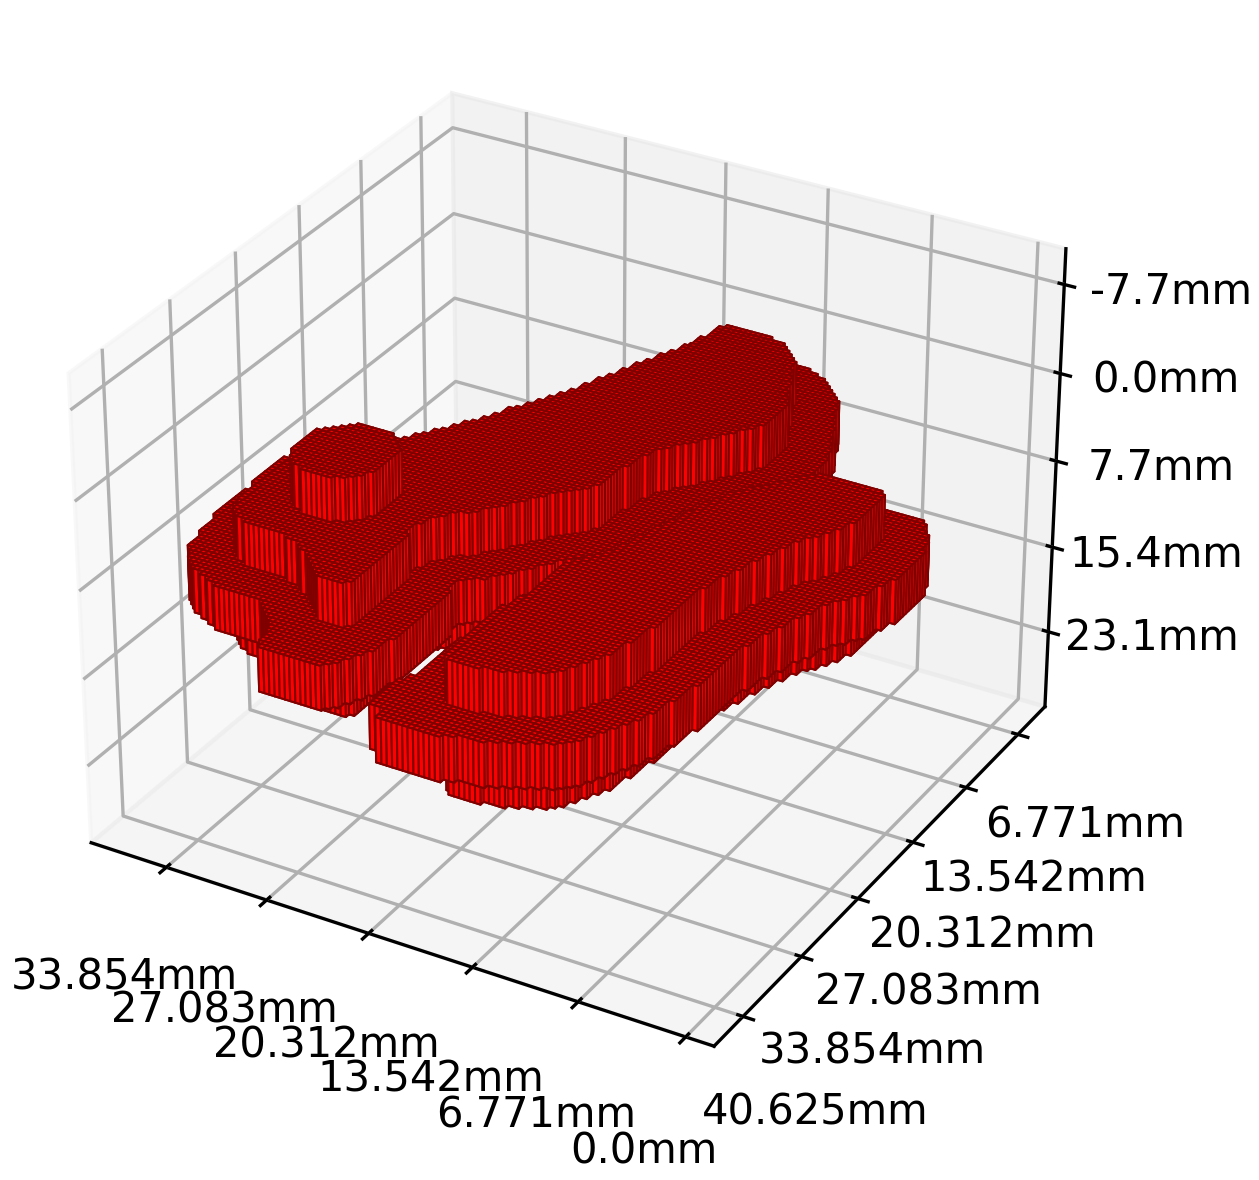
\includegraphics[width=\textwidth]{img/3d_mr1a.png}
        \caption{A 3-dimensional plot of the annotation. Note the uneven resolutions along different axes.}\label{fig:3d-3d}
    \end{subfigure}
    ~
    \begin{subfigure}[t]{0.4\textwidth}
        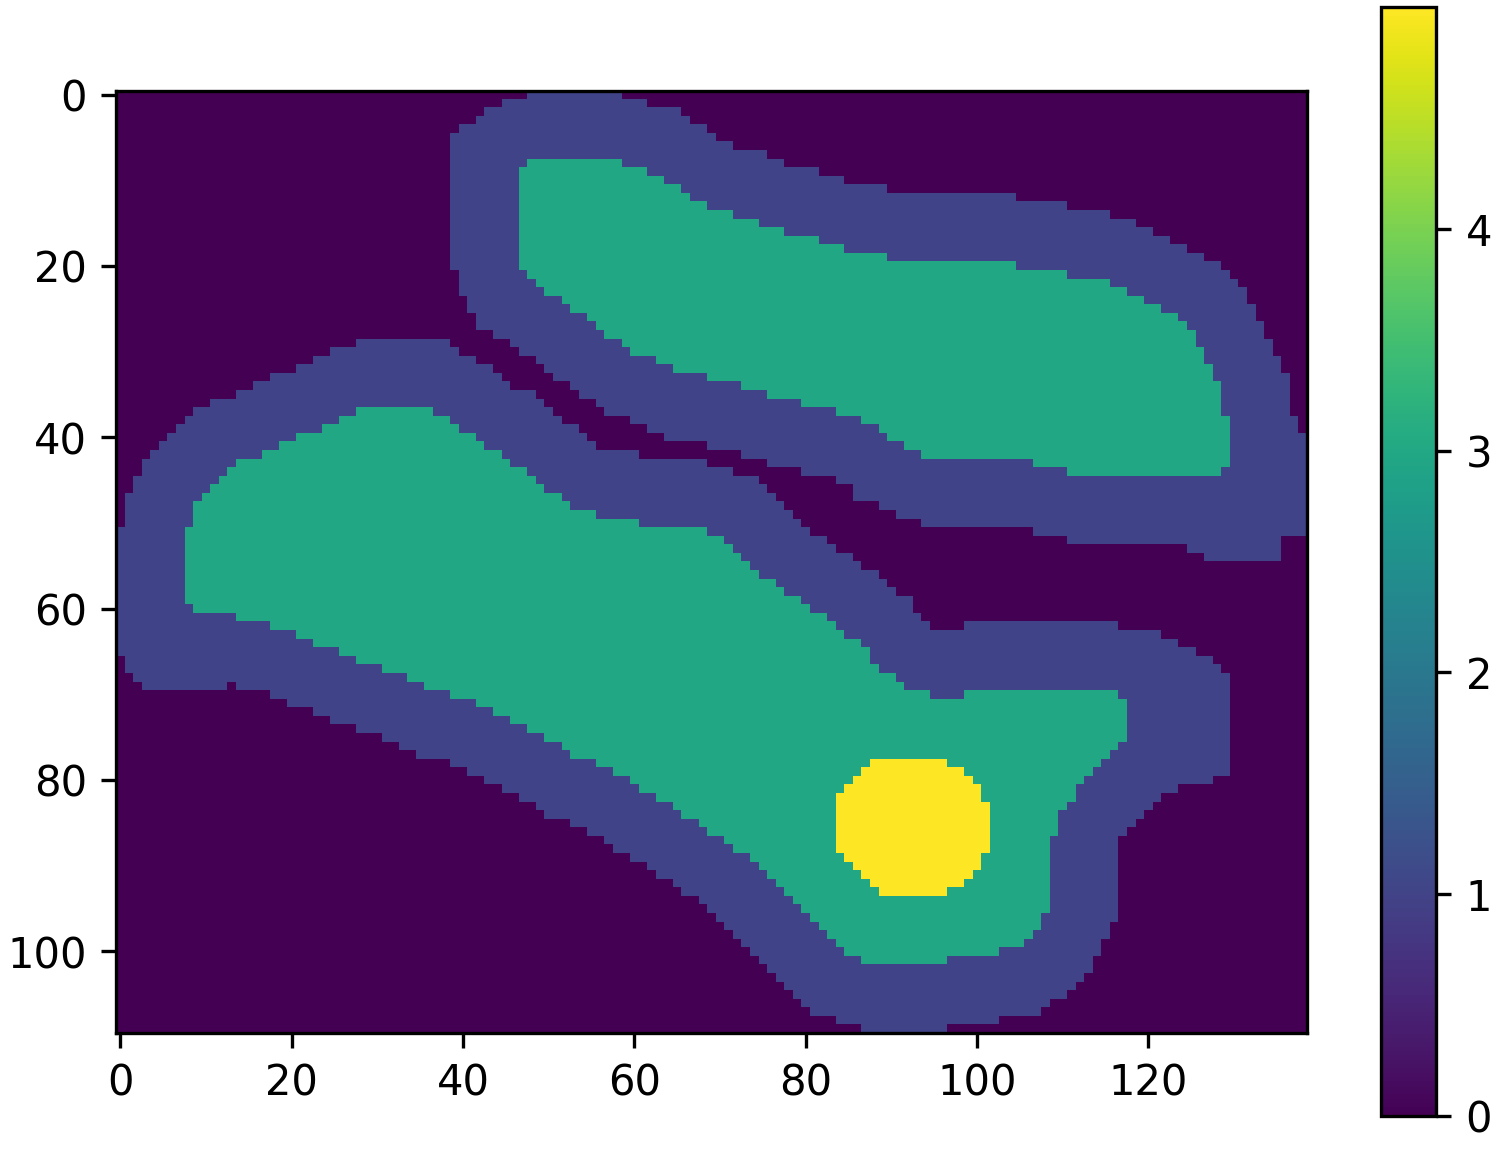
\includegraphics[width=\textwidth]{img/heatmap_mr1a.png}
        \caption{The 3-dimensional annotation projected back onto the original 2-dimensional annotation. The shape is symmetrical along the 2-dimensional base layer.}\label{fig:3d-2d}
    \end{subfigure}
    \caption{The 3-dimensional annotation generated from a 2-dimensional annotation. Both plots are cropped to the \ac{roi}.}\label{fig:3d-annotation}
\end{figure}

\subsubsection{Optimization of 3D-reconstruction}

The algorithm described above is inefficient for large images. 
Its complexity can be described by $\mathcal{O}(n~\cdot~m)$, where $n$ is the 
total number of voxels in the new annotation and $m$ is the number 
of voxels (or pixels, as it only uses two axes) in the original 2-dimensional
annotation. As tumors (and therefore tumor annotations) cover only small 
parts of the total 3D image, most pixels in the new annotation ($n$) are 
checked\footnote{\enquote{Checked} refers a voxel's distance to a pixel 
in the original annotation being calculated and compared to that pixel's 
\enquote{2D-distance}.} for no reason; the distance of the majority of 
voxels to the \ac{roi} is far greater than the \enquote{2D-distance} 
of any pixels in the original annotation.

The following changes in the algorithm defined earlier aim to reduce the
amount of unnecessary distance measurements. Instead of checking every
new voxel in the new annotation for its distance to a pixel in the original
annotation, a cube of influence is calculated for that pixel. In the center
of this cube of influence lies a pixel in the original annotation. The 
size of the cube is determined by the pixel's \enquote{2D-distance}; 
the \enquote{2D-distance} is divided by each axis' scale. This, rounded down
to the next whole number, gives the \enquote{radius} of the cube along
each axis. For example, a pixel may possess a \enquote{2D-distance} of
10 mm. For axis scales of 3 mm, 3 mm and 12 mm, the cube of influence would
measure 7$\times$ 7$\times$ 1 voxels. These dimensions result from the 
radii (3, 3, 0) being applied in both directions (e.g. \enquote{forward} 
and \enquote{backward}) and the initial voxel being added in the center. 
Each voxel in this cube is now checked to be closer to the original pixel
than the pixel's \enquote{2D-distance}. If so, the voxel is added to the 
new annotation. Should the voxel already be part of the new annotation 
(because it was already assigned this value through comparison to an
earlier pixel), it is not checked again.

\subsubsection{Rationalization}

As of time of writing, the (semi-)automatic segmentation of tumors is 
a problem without a generally agreed-on solution. Current approaches include
\ac{dl} based approaches such as~\cite{u-net_auto_anno} and~\cite{dl_rectal_segmentation}. 
To train \ac{dl} models accurately, a certain amount of input data is required, both as ground
truth and training data. In~\cite{u-net_auto_anno}, 300 3-dimensionally annotated \ac{mri} scans
are used for training, validation and testing, while~\cite{dl_rectal_segmentation} uses
a total of 140 scans. These quantities of scans far outweigh the total count of 5 3-dimensionally 
annotated scans available here.

Another common approach is semi-automatic segmentation. \cite{auto_and_semiauto} proposes 
both an automatic and a semi-automatic method of segmentation. While lightening the burden on
medical professionals, both of these methods rely on prior medical knowledge, or at the 
very least, human interaction. As the relevant medical information is not available in
this project, no approach described by~\cite{auto_and_semiauto} can be utilized.
Different semi-automatic segmentation methods, even if they may not depend on any medical
training, are still, by definition, based on human interaction. As one the main goals
of the 3D-reconstruction described here is to be easily reproducible, introducing a 
human factor may be detrimental this objective.

% Semiauto - not feasable due to missing medical knowledge.
% Therefore going for a "good-enough" method. Reference both automatic and semi-automatic methods of "Automated and Semiautomated Segmentation of Rectal Tumor Volumes on Diffusion-Weighted MRI: Can It Replace Manual Volumetry?" as both require human intervention
% 3D tumors seems to be round-ish. Maybe look for more data confirming or confute this.

% Optimization: Could you just cut down (empty) new annotation to size
% of old annotation (make square of 2D to cube)
% Implement ^this, benchmark both, use faster. Describe benchmark in paper
% NVM, ^this is still O(n*m), while per-pixel cube approach still skips
% most n pixels

% Maybe count distance measures in original and optimized method and 
% plot both?

% For results/improvement: Describe why balanced accuracy and not overall accuracy
% is important for unbalanced dataset

\section{Machine Learning Model}

As mentioned earlier, the main goal of this work is to, with reasonable 
accuracy, predict the \ac{pcr} of a patient. Essentially, this creates a 
question of \enquote{Yes} or \enquote{No}. A process assigning its input data to 
one of two categories can be represented as a two-class classifier. 

The classifier chosen here is the \enquote{Random Forests} model. If offers 


\subsection{Implementation}

\texttt{sklearn} offers an implementation of a random forest classifier through
its \\\texttt{sklearn.ensemble.RandomForestClassifier} class. This implementation
was chosen for a host of reasons. Being written in Python, it offers a 
accessible and easy to use interface and compatibility with other feature-rich
data analysis tools (such as, but not limited to, \texttt{numpy}, 
\texttt{pandas} and \texttt{matplotlib}). Additionally, being an open-source
project, the library is both cheap (i.e.~free) to acquire and use 
(assuming no license violations) and easy to version and distribute, increasing 
reproducibility. 



\subsection{Model Selection}
% Why random forest and why in sklearn?

\subsection{Training}
% Sample functions and parameters

\subsection{Feature Filtering}

With an input vector of 1743 features, it is not expected that each feature 
affects the final classification decision equally, or at all. 
A list of the \enquote{importance} of each feature, i.e.~the impact its value 
will have on that final decision, can be generated after a random forest is 
built.

From this list of importances we can see, that a significant portion of our 
input data has very little importance in our model. Although not helpful for our 
purpose, these features still must be considered in building our random forest 
and may be chosen to form decision trees, introducing additional but ultimately 
pointless nodes into our decision trees. This may negatively impact the 
performance of the model~\cite{elements_of_statistical_learning}.
For this reason, features of low importance will be filtered out.

\subsubsection{Determining Importance}

The choice of training and testing inputs determine the resulting model, the 
importance of individual features and its (balanced\footnote{Unless explicitly
stated otherwise, all mentions of \enquote{accuracy} refer to \enquote{balanced
accuracy}.}) accuracy. As the input sets are split randomly, both the accuracy
of the model and features' contributions to the result may vary strongly.

To avoid basing the decision about a feature's relevancy to the overall result
by a single model, which may represent an outlier, the importance is determined
by a weighted average over multiple models. To reduce the impact inaccurate 
models on the total priority of features, each model is weighted by its 
accuracy, adjusted to conform to a range of \enquote{0} to \enquote{1}, for 
the worst and best possible result respectively. Assuming the importance of 
a feature is calculated over \(m = 100\) models, where \( b_n \) is the 
(adjusted) accuracy of model \(n\) and \(i_n\) is the importance of this 
specific feature in this specific model, the weighing can be described as in
Equation~\ref{eq:weighted_average}.

\begin{equation} \label{eq:weighted_average}
    \sum_{i=1}^{m} \frac{b_n \cdot i_n}{m}
\end{equation}

When applied to all available features, the resulting importance distribution
can be seen in Figure~\ref{fig:importance_dist}. Note the peak at, or near, 
zero.

\begin{figure}[H]
    \centering
    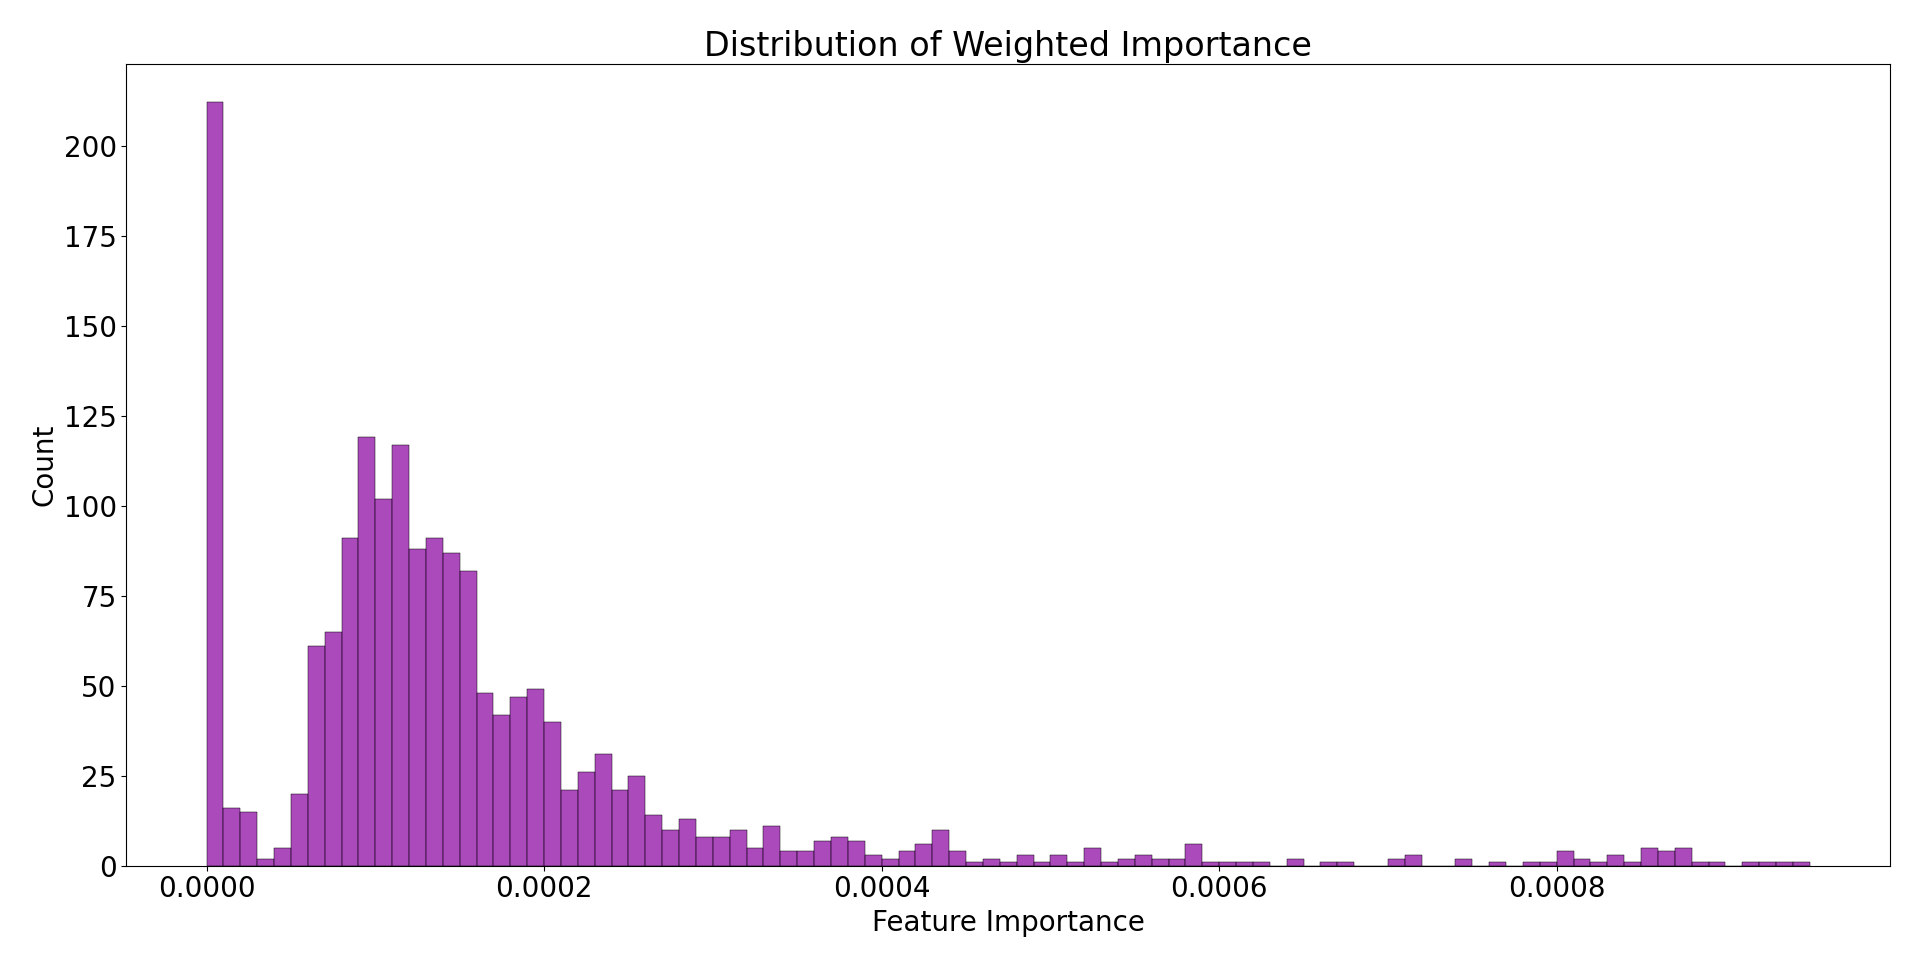
\includegraphics[width=\textwidth]{img/feature_importance_dist.png}
    \caption{Amount of fe.}\label{fig:importance_dist}
\end{figure}

\subsubsection{Filter Levels}

With a set of weighted importances, a filter can be created. This filter drops
all features with an importance below a certain level. A filter has been applied
for a 100 equally distributed levels between \enquote{0} and the maximum 
importance in the list of weighted importances. For each of these filters, the
average over a 100 models has been calculated, the results of which can be seen
in Figure~\ref{fig:importance_filter}.

\begin{figure}[H]
    \centering
    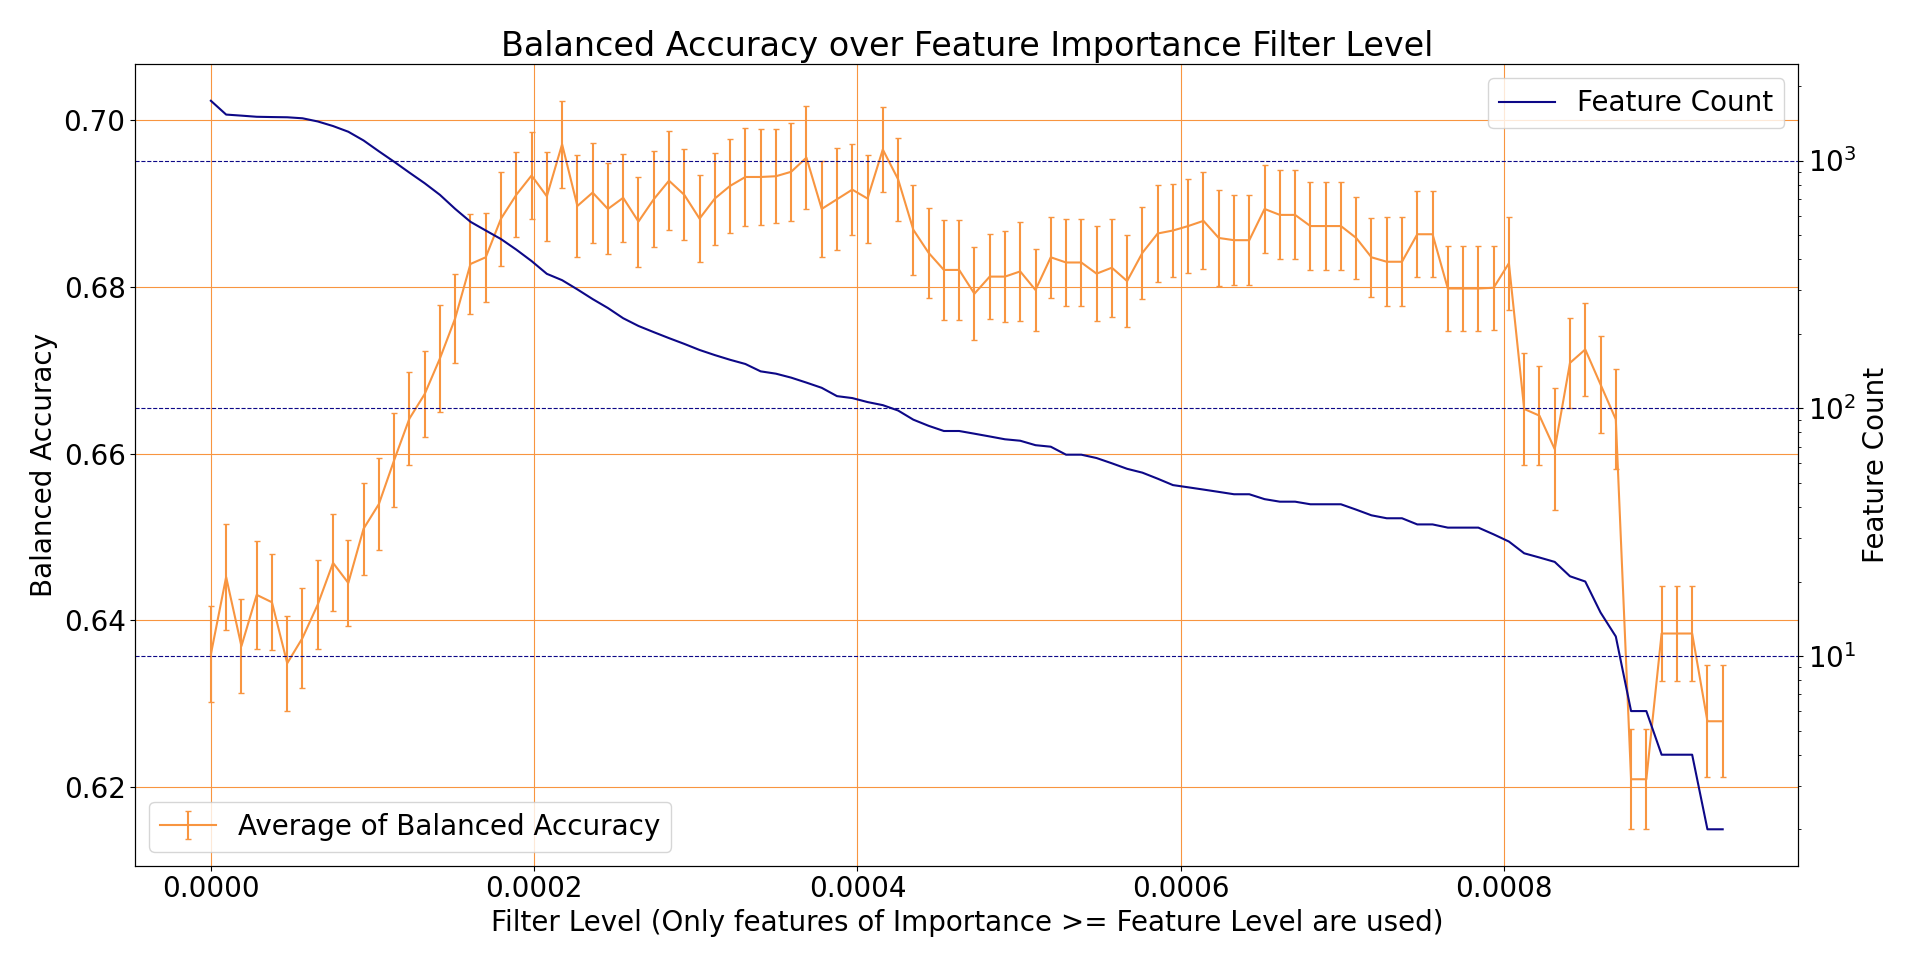
\includegraphics[width=\textwidth]{img/filter_levels_accuracy_logcount.png}
    \caption{Amount of feature per model, accuracy and variance of accuracy of 
    this model over the filter level. Note the logarithmic y-axis for Feature Count.}\label{fig:importance_filter}
\end{figure}

Without filtering, the accuracy of the model sits at a base level of 
0.6359. Removing zero to very low importance features initially barely improves
accuracy. 
% Improvements to ~0.66 start at 0.000251708540042472 with 1057 features. Note, this is the flawed run, correct his after new run.
% TODO: Analyze the results further

\subsection{Evaluation}
% Not exactly sure yet.
% If applicable, show process of selecting important radiomics features

\section{Results}
% Hopefully, one day

\section{Discussion}
% Optionally, if there's something interesting to say about the results. 
% Maybe compare to similar paper.